\documentclass[12pt]{article}
\usepackage[margin=1in]{geometry}
\usepackage{setspace}
\onehalfspacing

% Start of preamble
%==========================================================================================%
% Required to support mathematical unicode
\usepackage[warnunknown, fasterrors, mathletters]{ucs}
\usepackage[utf8x]{inputenc}

\usepackage[dvipsnames,table,xcdraw]{xcolor}

% Standard mathematical typesetting packages
\usepackage{amsmath,amssymb,amscd,amsthm,amsxtra, pxfonts}
\usepackage{mathtools,mathrsfs,dsfont,xparse}

% Symbol and utility packages
\usepackage{cancel, textcomp}
\usepackage[mathscr]{euscript}
\usepackage[nointegrals]{wasysym}
\usepackage{apacite}

% Extras
\usepackage{physics}  
\usepackage{tikz-cd} 
\usepackage{microtype}
\usepackage{enumitem}
\usepackage{titling}
\usepackage{graphicx}

% Fancy theorems due to @intuitively on discord
\usepackage{mdframed}
\newmdtheoremenv[
backgroundcolor=NavyBlue!30,
linewidth=2pt,
linecolor=NavyBlue,
topline=false,
bottomline=false,
rightline=false,
innertopmargin=10pt,
innerbottommargin=10pt,
innerrightmargin=10pt,
innerleftmargin=10pt,
skipabove=\baselineskip,
skipbelow=\baselineskip
]{mytheorem}{Theorem}

\newenvironment{theorem}{\begin{mytheorem}}{\end{mytheorem}}

\newtheorem{corollary}{Corollary}
\newtheorem{lemma}{Lemma}

\newtheoremstyle{definitionstyle}
{\topsep}%
{\topsep}%
{}%
{}%
{\bfseries}%
{.}%
{.5em}%
{}%
\theoremstyle{definitionstyle}
\newmdtheoremenv[
backgroundcolor=Violet!30,
linewidth=2pt,
linecolor=Violet,
topline=false,
bottomline=false,
rightline=false,
innertopmargin=10pt,
innerbottommargin=10pt,
innerrightmargin=10pt,
innerleftmargin=10pt,
skipabove=\baselineskip,
skipbelow=\baselineskip,
]{mydef}{Definition}
\newenvironment{definition}{\begin{mydef}}{\end{mydef}}

\newtheorem*{remark}{Remark}

\newtheorem*{example}{Example}

% Common shortcuts
\def\mbb#1{\mathbb{#1}}
\def\mfk#1{\mathfrak{#1}}

\def\bN{\mbb{N}}
\def \C{\mbb{C}}
\def \R{\mbb{R}}
\def\bQ{\mbb{Q}}
\def\bZ{\mbb{Z}}
\def \cph{\varphi}
\renewcommand{\th}{\theta}
\def \ve{\varepsilon}
\newcommand{\mg}[1]{\| #1 \|}

% Often helpful macros
\newcommand{\floor}[1]{\left\lfloor#1\right\rfloor}
\newcommand{\ceil}[1]{\left\lceil#1\right\rceil}
\renewcommand{\qed}{\hfill\qedsymbol}
\renewcommand{\P}{\mathbb P\qty}
\newcommand{\E}{\mathbb{E}\qty}
\newcommand{\Cov}{\mathrm{Cov}\qty}
\newcommand{\Var}{\mathrm{Var}\qty}

% Sets
\usepackage{braket}

\graphicspath{{/}}
\usepackage{float}

\newcommand{\SET}[1]{\Set{\mskip-\medmuskip #1 \mskip-\medmuskip}}

% End of preamble
%==========================================================================================%

% Start of commands specific to this file
%==========================================================================================%

%==========================================================================================%
% End of commands specific to this file

\title{CSE 446 HW4}
\date{\today}
\author{Rohan Mukherjee}

\begin{document}
    \maketitle
    \subsection*{A1.}
    \begin{enumerate}[label=\alph*.]
        \item If the vectors are already lying in a $k$ dimensional subspace, then PCA will give us the matrix that projects onto that $k$ dimensional subspace. Since projecting a vector onto a subspace that it already lives in will just return the same vector, we see that the projection of the data onto the subspace will be just the data itself. Thus we have a 0 reconstruction error.
        \item False. The columns of $V$ are the eigenvectors of $X^TX$, not the rows. 
        \item False. Choosing $k$ to minimize the $k$ means objective does give good clusters for the data, but in the examples below, I got a lot of 9s in the 10 clusters and no 4s. 
        \item False. The SVD of a matrix is in general not unique. We could permute the columns of $U$, rows of $V$, and entries of $S$ (by the same permutation) to get another singular value decomposition. 
        \item False. Consider the matrix $aI \in \R^{n \times n}$ for some nonzero constant $a \in \R$. This matrix obviously has rank $n$, being invertible (with inverse $a^{-1} I$), but this matrix has only one eigenvalue $a$.
    \end{enumerate}

    \newpage
    \subsection*{A2.}
    \begin{enumerate}[label=\alph*.]
        \item The first thing I would do, like always, is to normalize the data by making the features have mean 0 and variance 1. Since we want to create an algorithm that learns the factors that contribute most to acquiring a specific disease, we want a relationship that puts weights on each of the factors and outputs the probability of having the disease. We can thus use binary logistic regression for this problem, because we want to predict if a person has a disease or not. The inputs in the weight vector will tell us which factors cause the disease. 
        
        We are left with a few questions. The first problem is that the logistic regression model might get bad accuracy on the validation set. This is extremely hard to get around--the main way to get around this is to allow non-lineararity in the model using multi-layered neural networks, but then we can't explain which factors cause the disease. Similarly, if we have a very small amount of training data, but an enormous amount of factors, we will almost surely overfit to the training data, leading to poor generalization. The last thing is that we could have completely nonsense features that certainly don't cause the disease, but show up as hugely positive weights in the model. For example, one of the features could be the number of times the person has been to the moon, which is obviously not a factor in acquiring the disease. Finally, given the limited amount of personal data from the person, you can put their data into the model and get a prediction of whether they have the disease or not. 

        \item The main potential shortcoming for my model having different accuracy on different populations is that if a lot of the training data is only on a specific population, say in a specific country, then the model won't really use that all the people are living in that one country, because it can't gain much information from a feature with really small variance. Then when another population comes around, whose disease susceptibility is really correlated with what country they live in, the model will have very bad accuracy on that data. The way to fix this is to get a more diverse training set, with people from all over the world. We could also use cross validation to train the model on different populations at a time and see if it generalizes well to the other populations. 
        
        \item Some real world implications that would come from ignoring the issues described in the question is again the problem of correlation and causation. Police might spend a lot more time patrolling a more dangerous neighborhood, so the crime statistic will be higher along with the police patrol being higher. From the above, one would say that it must be that police patrols cause crime, which is not true and again the problem of correlation vs causation. If many of the shortcomings such as crimes being reported at higher rates in minority neighborhoods, the model might put high weight on the minority percentage in a community and hence one might conclude that being a minority is the reason for crime. This is a problem of the model and a shortcoming of trying to interpret numbers like this in a real world setting. 
    \end{enumerate}

    \newpage
    \subsection*{A3.}
    \begin{enumerate}[label=\alph*.]
        \item Here is the graph of the training epoch vs accuracy, for the best 3 performing models:
        \begin{figure}[H]
            \centering
            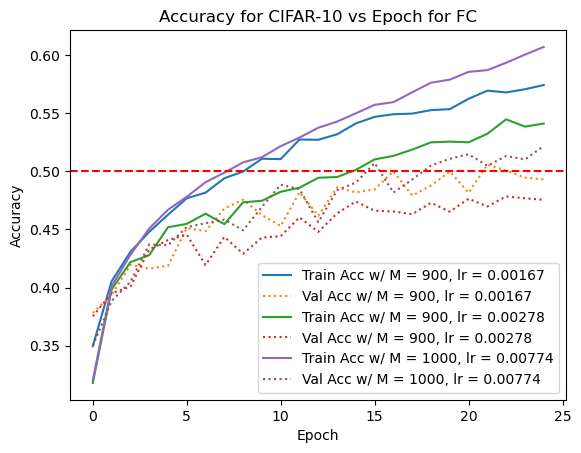
\includegraphics[width=0.7\textwidth]{FC_acc.png}
            \caption{Training epoch vs accuracy}
        \end{figure}
        For this first model, I used random search with $30$ iterations over learning rates in a logspace from $10^{-3}$ to $10^{-1}$, the M's were in a linspcae from $10$ to $1000$ and the momentums were in a linspace from $0.9$ to $0.99$, each with 10 elements in the range. I thought it would be best to have 10 iterations per hyperparameter. The best performing model as seen above has $M=1000$ with learning rate of $0.00774$. It had a test accuracy of $0.5178$.

        \item Here is the graph of the training epoch vs accuracy for the best 3 performing models for the convolutional neural network:
        \begin{figure}[H]
            \centering
            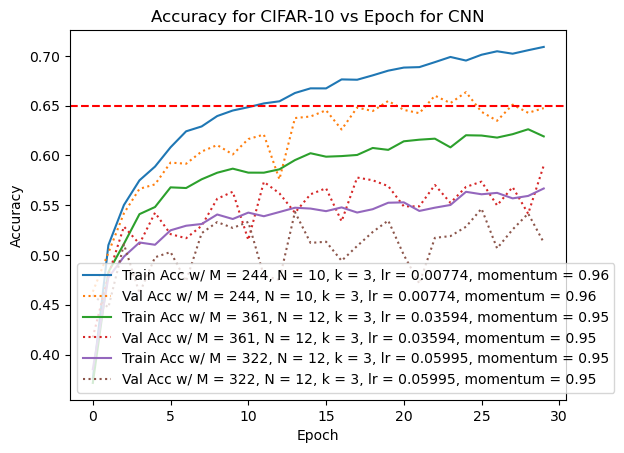
\includegraphics[width=0.7\textwidth]{CNN_acc.png}
            \caption{Training epoch vs accuracy}
        \end{figure}
        I used random search over these parameters:
        \begin{verbatim}
            lrs = np.logspace(-3, -1, 10)
            Ms = np.linspace(50, 400, 10).astype(int)
            Ns = np.linspace(10, 20, 5).astype(int)
            ks = np.linspace(2, 8, 5).astype(int)
            Momentums = np.linspace(0.9, 0.99, 10)
        \end{verbatim}
        The best performing model got an accuracy of 0.66317 on the test data, with hyperparameters $M=244$, $N=10$, $k=3$, $lr=0.00774$ and $momentum=0.96$.

        

    \end{enumerate}
    
    \newpage
    \subsection*{A4.}
    The image representing the 10 clusters is shown below:
    \begin{figure}[H]
        \centering
        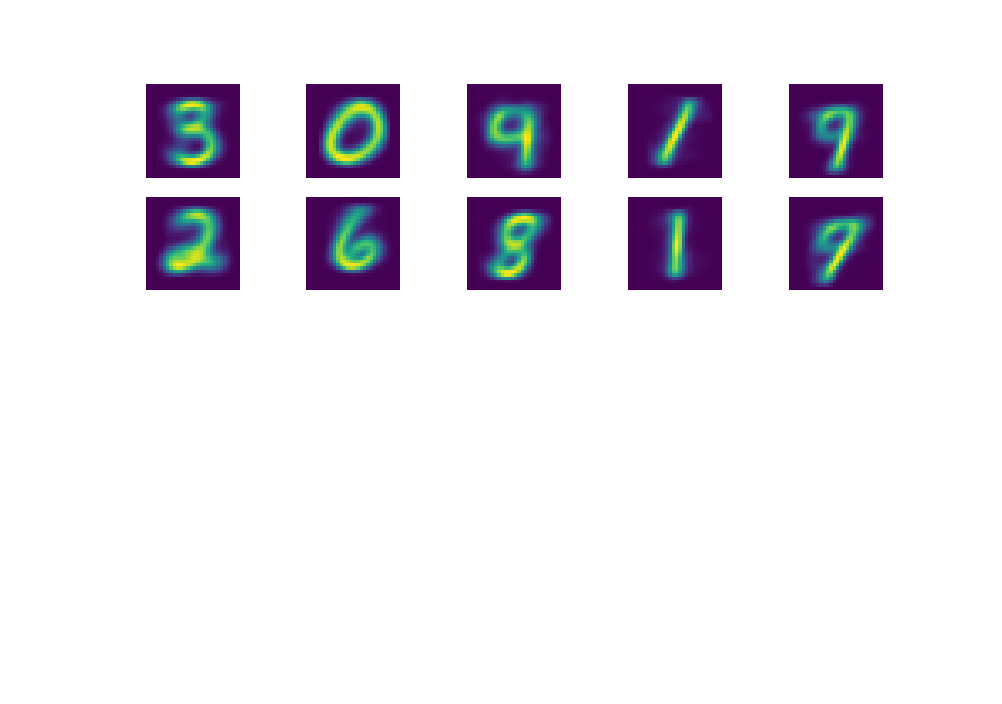
\includegraphics[width=0.7\textwidth]{clusters.png}
        \caption{Clusters of the data}
    \end{figure}

    \newpage
    \subsection*{A5.}
    I spent around 15 hours on this assignment. Training the models was the most time consuming part of the assignment as the Ed Discussion hinted at. Coding in pytorch is really fun, because it makes everything so simple. 
\end{document}